\documentclass[a4paper,12pt]{article}

% don't forget the document class, generally : \documentclass[a4paper,12pt]{article}

\usepackage[utf8]{inputenc}
\usepackage[french]{babel}
\usepackage{graphicx}
\usepackage{gensymb}
\usepackage{amsmath}
\usepackage{float}
\usepackage{scrextend}
\usepackage{caption} 
\usepackage{siunitx}
\usepackage{enumitem}
\usepackage{amsthm}
\usepackage{fancyhdr}
\usepackage{amssymb}
\usepackage{wrapfig}
\usepackage{geometry}
\usepackage{standalone}
\usepackage{import}
\usepackage[usenames, dvipsnames]{color}

 \usepackage{biblatex} % manages bibliography and references
\addbibresource{sample.bib}


\geometry{hmargin=1in, vmargin=1in}

 \newenvironment{absolutelynopagebreak}
 {\par\nobreak\vfil\penalty0\vfilneg
 \vtop\bgroup}
 {\par\xdef\tpd{\the\prevdepth}\egroup
 \prevdepth=\tpd}
 
 \pagestyle{fancy}                        
\fancyhf{}                               
\fancyhf[HL]{Application des maths}                
\fancyhf[HR]{Géométrie euclidienne}             
\fancyhf[FC]{\thepage/\pageref{Lastpage}}
 
\newtheorem{definition}{Définition}[section]
\newtheorem{theorem}{Théorème}
\newtheorem{corollary}{Corollaire}[theorem]
\newtheorem{lemma}[theorem]{Lemme}
\newtheorem*{hyp}{Hypothèse}
\newtheorem*{concl}{Conclusion}
\newtheorem*{remark}{Remarque}

\captionsetup{format=default,labelformat=simple,labelsep=colon,
justification=justified,font={sf,small},labelfont=bf,
textfont=default} 



\begin{document}

\pagebreak
\subsection{Théorème de Phytagore}
\begin{theorem}
Dans tout triangle rectangle, le carré de l'hypothénuse équivaut à la somme des carrés des deux autres côtés.\\
Réciproquement, un triangle dont le carré de l'hypothénuse équivaut à la somme des carrés des deux autres côtés est rectangle.
\end{theorem}


\begin{proof}
Nous considérons le triangle rectangle $\triangle ABC$.

\begin{hyp}
$\triangle ABC$ est rectangle en $\gamma$
\end{hyp}

\begin{concl}
c^2 = a^2 + b^2
\end{concl}




\end{proof}



\begin{remark}
Ce théorème porte le nom du fort célèbre mathématicien et philosophe Phytagore (voir figure  \ref{fig:pythagore} \footnote{Image disponible sur [dernière consultation: 5.12.2016]: http://data.abuledu.org/searchhtml.php?terms=Pythagore}). Voici ce que AS Montferrier écrit à son sujet en 1835, dans son "Dictionnaire des sciences mathématiques pures et appliquées".\\

"On ignore l’époque précise de la naissance de Pythagore, mais il résulte de toutes les controverses auxquelles cette question historique a donné lieu que ce grand homme vivait vers la fin du sixième siècle avant J.-C. Les témoignages de l’antiquité diffèrent également sur le lieu où il naquit, mais la plus commune opinion est qu’il reçut le jour à Samos. Cette île était alors dans un état florissant; elle étendait au loin ses relations commerciales, et il est permis de croire que ce fut d'abord en accompagnant Mnésarque, son père, qui exerçait le négoce, que Pythagore contracta le goût des voyages qu’il entreprit depuis dans un but
plus élevé. Sans doute, doué comme il l’était d’un esprit élevé, d’un amour ardent pour la vérité, possédant toute l'instruction qu’il était alors permis d’acquérir, Pythagore dut profiter, dans ses longs et nombreux pèlerinages, d’une foule de connaissances qu’il trouva chez des peuples plus anciens en civilisation que ses compatriotes. Mais il serait absurde d’attribuer à cette source les idées philosophiques et les découvertes dans l'arithmétique, la géométrie et l’astronomie qui n’appartiennent qu’à son génie.
[...]\\
Les vérités mathématiques formaient la branche la plus essentielle de l’enseignement de Pythagore. A part la découverte de la propriété du triangle rectangle, c’est-à dire la démonstration du carré de l’hypothénuse, on attribue avec raison à ce philosophe une foule de théories alors nouvelles, en géométrie, dont la vulgarisation a singulièrement contribué aux progrès de la science. Il résulte des différens [sic] rapports des écrivains de l’antiquité qui nous ont transmis ses opinions, qu’il avait les idées les plus justes sur les points fondamentaux de l’astronomie: ainsi il enseignait a [sic] ses disciples la distribution de la sphère céleste, l’obliquité de l’écliptique, la sphéricité de la terre et celle du soleil, la cause de la lumière de la lune, celle des éclipses de ces deux astres, et enfin le mouvement de la terre." \footnote{Montferrier, Alexandre Sarrazin. Dictionnaire des sciences mathématiques pures et appliquées. Vol.~2. Bibliotheque scientifique, 1835. Extrait de l'article \textit{Pythagore}, pages 386-389.}

\begin{figure}[H]\label{fig:pythagore}
    \centering
    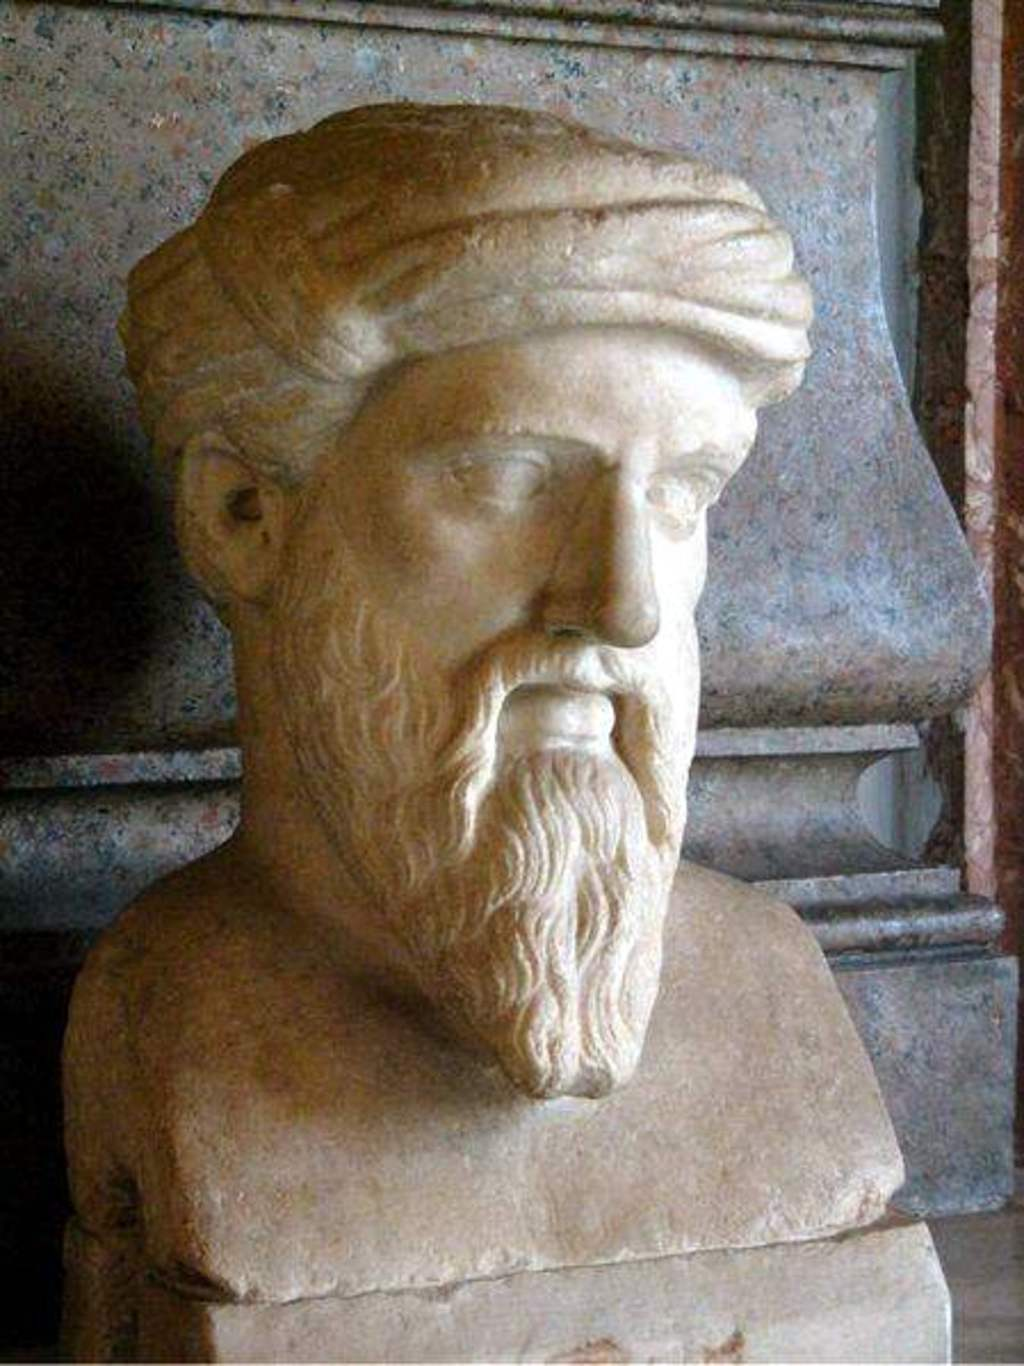
\includegraphics[scale=0.3]{theorems/pythagore/pythagore.jpg}
    
    \caption{Buste de Pythagore datant du $V^{me}$ siècle avant J.C.}
    \label{fig:thales}
\end{figure}

\end{remark}

\end{document}

